\section{Theorie}
\label{sec:theorie}

Ein Operationsverstärker ist definiert als ein elektronischer Verstärker, der gleichspannungsgekoppelt ist und einen hohen Verstärkungsfaktor besitzt.
Er kann benutzt werden, um verschiedene mathematische Rechenoperationen durchzuführen, wie Addieren, Subtrahieren, Differenzieren und Integrieren.\\
Der ideale Operationsverstärker hat zwei Eingänge und einen verstärkenden Ausgang, der unabhängig von äußeren Einflüssen einen gleichbleibenden Verstärkungsfaktor ohne Verluste besitzt.
Das Schaltzeichen dafür ist in \autoref{fig:symbol} dargestellt.

\begin{figure}[H]
    \centering
    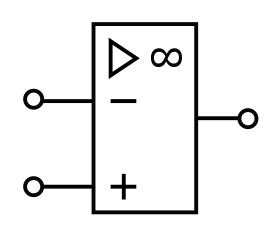
\includegraphics[scale=0.5]{images/symbol.png}
    \caption{Darstellung eines Operationsverstärkers nach DIN-EN-6067 Norm.\cite{V51}}
    \label{fig:symbol}
\end{figure}

Bei einem invertierenden Linearverstärker, dessen Schaltung in \autoref{fig:linear} dargestellt ist, beträgt der ideale Verstärkungsfaktor somit
\begin{equation}
    \nu = -\frac{R_2}{R_1}
\end{equation}

\begin{figure}[H]
    \centering
    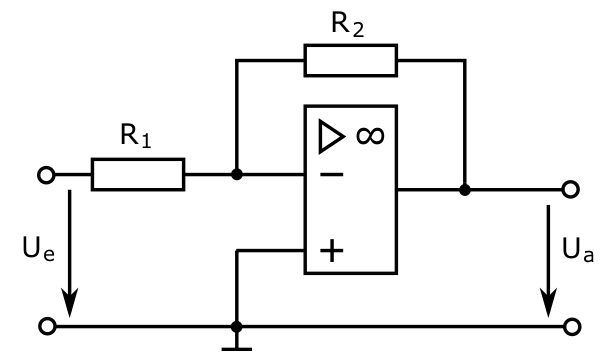
\includegraphics[scale=0.5]{images/linear.png}
    \caption{Aufbau eines invertierenden linearen Verstärkers.\cite{V51}}
    \label{fig:linear}
\end{figure}

Alle realen Operationsverstärker besitzen zusätzlich zum positiven und negativen Eingang noch zwei Eingänge für die Versorgungsspannung.
Diese werden typischerweise mit $U_{CC}$ und $U_{EE}$ bezeichnet und mit $\pm$\SI{15}{\volt} belegt.\\
Dabei ist es wichtig die Versorgungsspannung symmetrisch zu wählen, da diese das Ausgangssignal beeinflusst.
Der Operationsverstärker besitzt eine Saturierungsspannung, die vorgibt, wie hoch $U_A$ in Abhängigkeit von $U_{CC,EE}$ sein kann.
In \autoref{fig:satur} ist das graphisch dargestellt.

\begin{figure}[H]
    \centering
    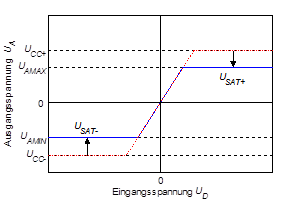
\includegraphics[]{images/satur.png}
    \caption{Dieser Graph zeigt den Verlauf der Ausgangsspannung bei anliegender Eingangsspannung in Abhängigkeit der Versorgungsspannung an.
    Es ist zu erkennen, dass die Saturierungsspannung $U_{SAT}$ die Ausgangsspannung abhängig von der Versorgungsspannung betragsmäßig verringert.\cite{satur}}
    \label{fig:satur}
\end{figure}

Die Formel zur Berechnung der Ausgangsspannung ist:
\begin{equation}
    \begin{aligned}
        U_{A,max} = U_{CC} - U_{SAT+}\\
        U_{A,min} = U_{EE} - U_{SAT-}
    \end{aligned}
\end{equation}
Daraus geht hervor, dass eine unsymmetrische Versorgungsspannung zu einer unsymmetrischen Ausgangsspannung führt, was für einen Betrieb mit Wechselspannung unerwünschte Effekte zur Folge hat.\\

\subsection{Invertierender Linearverstärker}
Der invertierende Linearverstärker wurde bereits in \autoref{fig:linear} dargestellt.
Die Verstärkung ist nicht konstant, wie bei einem idealen Verstärker, sondern nimmt bei steigender Frequenz der Eingangsspannung ab.
Der Übergang von konstanter Verstärkung zu abfallender Verstärkung ist ab der Grenzfrequenz $f_{grenz}$ erkennbar.
